\documentclass{article}
\usepackage[english]{babel}
\usepackage[utf8]{inputenc}
\usepackage[colorlinks]{hyperref}
\usepackage{enumitem,kantlipsum}
\usepackage{graphicx, color}
\usepackage{amsfonts}
\newcommand{\TODO}[1]{ {\color{blue} #1 }}
\newtheorem{proposition}{Proposition}


\title{{\Huge PACT\/}:   {\Huge P\/}rivacy Sensitive Protocols {\Huge A\/}nd Mechanisms
\\for Effective Mobile {\Huge C\/}ontact {\Huge T\/}racing }
\date{}

\setlength{\oddsidemargin}{0.25 in}
\setlength{\evensidemargin}{-0.25 in}
\setlength{\topmargin}{-0.6 in}
\setlength{\textwidth}{6.5 in}
\setlength{\textheight}{8.5 in}
\setlength{\headsep}{0.75 in}
\setlength{\parindent}{0 in}
\setlength{\parskip}{0.1 in}


\newcommand{\sk}[1]{\textsf{\color{magenta} SK: #1}}

\begin{document}

\maketitle

\begin{abstract}
The global health threat from COVID-19 has been controlled in a number of instances by large scale testing and contact tracing efforts.
Our goal is to develop contact tracing approaches which harness computing technologies which support the goals of public health organizations, while protecting the civil liberties of individuals.  We note that there are an increasing number of contact tracing applications being released with different protocols, all under an umbrella of  ``privacy preserving".  In addition to just understanding privacy, it is equally important to consider inferential risks, where any alert to a user could itself give rise to de-anonymizing information.  
%Any protocol that seeks broad adoption must transparently presnt 

%and the population overall to minimize morbidity and mortality associated with the spread of COVID-19.  
%We focus on privacy-sensitive methods and protocols that avoid the use of a trusted third party through the use of mobile tracing applications that assist and augment existing manual contact tracing efforts.  

This work considers three functionalities assisting mobile contract tracing, and sets forth transparent privacy and anonymity standards,
where the goal is to permit adoption of mobile contract tracing efforts while upholding civil liberties.  The protocols we advocate for are a third-party free approach, because such an approach mitigates security and privacy risks due to assuming the third party is trustworthy. We also 
hope to bring together multiple communities to develop acceptable, interoperating, protocols which support mobile contact tracing applications in a privacy-sensitive manner.
\end{abstract}

\iffalse
\emph{Our goal is to bring together colleagues in industry, academia, and civil society to discuss and converge on ideas around a critical issue rising with attempts to mitigate the COVID-19 pandemic.  This work advocates for a third-party free approach to assisted mobile contact tracing, because such an approach mitigates security and privacy risks. More generally, this document espouses the view that discussion of ``privacy'' need to directly consider the inferential risks of re-identification. Furthermore, we make a case that to best assist public health organizations, further functionalities should be considered. We hope that this collaborative effort helps us converge on best practices on protocols and implementations across a set of a multiparty stakeholders.
% Pressures to perform testing and tracing to control the spread of the virus threaten our civil liberties. 
%Early implementations have been imposed by authoritarian and democratic regimes.  
%This document was created to promote discussion on how we might best harness computing technology to protect the civil liberties of individuals, while supporting the goals of public health organizations and the population overall to minimize morbidity and mortality associated with the spread of COVID-19. 
%We focus on privacy-sensitive methods and protocols that could be employed with any mobile tracing applications. 
%We hope to bring together multiple communities to develop acceptable, interoperating, protocols which support mobile contact tracing applications in a privacy-sensitive manner, even if the details differ. We note that there are an increasing number of contact tracing applications being released with different protocols (see Section~\ref{sect:apps}), where it is difficult for the user to interpret what ``privacy" means. 
}
\fi

\iffalse
This is an evolving document. Our goal is to bring together colleagues in industry, academia, and civil society to discuss and converge on ideas around a critical issue rising with attempts to mitigate the COVID-19 pandemic. Specifically, pressures to perform testing and tracing to control the spread of the virus threaten our civil liberties. Early implementations have been imposed by authoritarian and democratic regimes.  We created this document to promote discussion on how we might best harness computing technology to protect the civil liberties of individuals, while supporting the goals of public health organizations and the population overall to minimize morbidity and mortality associated with the spread of COVID-19. We focus on privacy-sensitive methods and protocols that could be employed with any mobile tracing applications. We hope to bring together multiple communities to develop acceptable, interoperating, protocols which support mobile contact tracing applications, even if the details of the approaches differ. We note that there are an increasing number of contact tracing applications being released with different protocols, some without privacy considerations and others where it is difficult to interpret what "privacy" means. We hope that this effort will help us to converge on best practices on protocols and implementations as a set of a multiparty stakeholders.
\fi

\iffalse
\begin{figure}
\begin{center}
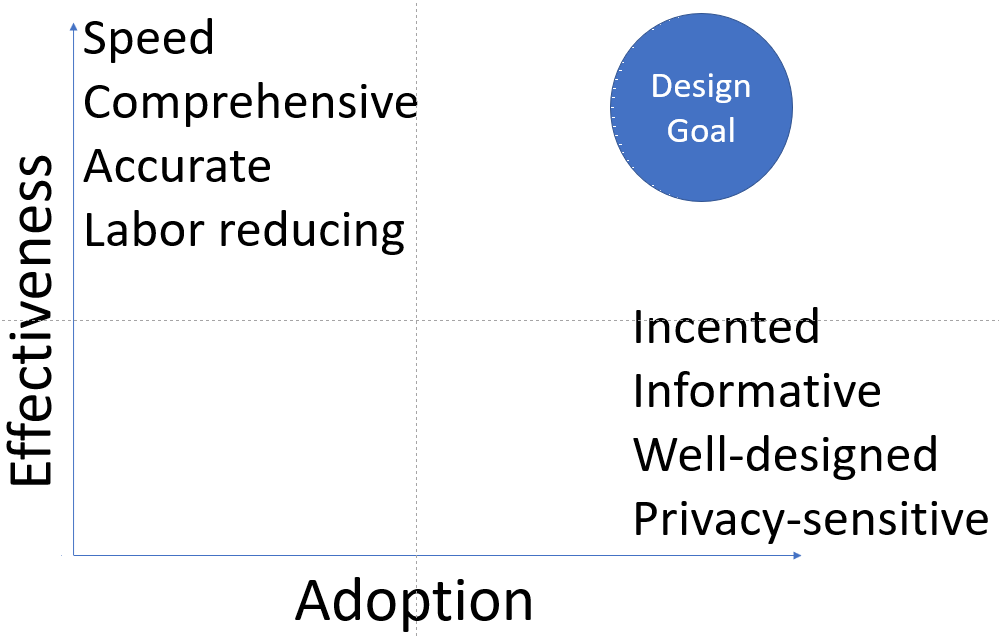
\includegraphics[scale=0.25]{Design_Goal}
\end{center}
\caption{\label{fig:design_goal}Design goals for a successful mobile contact tracing app.}
\end{figure}
\fi

As nations are seeking to circumvent devastating death tolls from COVID-19, many are resorting to \emph{mobile-based, contact tracing technologies} as a key tool in mitigating or suppressing the pandemic. Harnessing mobile computing technologies is an obvious means to dramatically scale-up conventional epidemic response contact tracing strategies to much greater scale than has ever before been used.  Notably, South Korea managed to successfully suppress a large outbreak using this strategy.  

\iffalse
Conducting mobile contact tracing effectively requires a strategy which maximizes adoption and epidemiological effectiveness as depicted in figure~\ref{fig:design_goal} which shows two critical axes.   On the medical effectiveness axis, we want an approach that: speeds up the process of contact tracing; creates more comprehensive contact tracing interviews; is more accurate than existing contact tracing, and reduces the labor of doing contact tracing.  On the adoption axis, you want to incentivize wide adoption, have an app which is informative to the user to keep that adoption, have it be well-designed so users can benefit form it, and to respect the privacy and autonomy of the user.  There are presently many approaches proposed (see section~\ref{sec:alternatives}) or fielded (see section~\ref{sect:apps}).  For example, some of these make severe choices against adoption by neglecting the civil liberties that citizens expect and demand implying they are simply not of interest to voluntary users.  

We believe it is possible to largely avoid tradeoffs allowing the creation of an  epidemiologically effective app that empowers all participants.  Here, we primarily focus on the design of privacy sensitive approaches which are also medically effective.  Other adoption-related issues are of course important, but appear less central to the core information architecture of the system. 
\fi

Many proposed or fielded protocols rely on a government or a trusted 3rd party to gather  information from participating phones, do analysis, and announce results to various parties.  Although this approach is straightforward, many people naturally oppose the aggregation of information and power that it represents as well as the precedent it sets. 
%Given this, we expect resistance to these approaches leading to low adoption.  
This work considers 3rd party free approaches which keep the data and compute on the phones, creating an approach which respects civil liberties and the privacy of participants.  In cases where it is valuable for individuals to share data with others, this approach provides voluntary mechanisms in accordance with ethical principles of personal decision making, including disclosure, and consent.  We refer to efforts to identify, study, and field such privacy-sensitive technologies, architectures, and protocols in support of mobile tracing as PACT (\emph{P}rivacy sensitive protocols \emph{A}nd standards for mobile \emph{C}ontact \emph{T}racing).

\begin{center}
\emph{The objective of PACT is to set forth transparent privacy and
  anonymity standards,\\
  which permit adoption of mobile contract tracing efforts while upholding civil liberties.}
\end{center}

We seek to specify a set of protocols and standards that achieve
these objectives. We also wish to provide a means to support the use over a population of multiple, mobile contact tracing applications (running on different phones) via providing interoperating capabilities that assure consistency with regards to the goals of privacy. 

Conventional contact tracing strategies executed by public health organizations operate as follows: Positively tested citizens are asked to reveal (voluntary, or enforced via public health policy or by law depending on region) their contact history to public health officers. The public health officers then inform other citizens who have been at risk to the virus based on co-location, via some definition of co-location, supported by look-up or inference about locations. The citizens deemed to be at risk are then asked to take appropriate action (often to either seek tests or to quarantine
themselves and to be vigilant about symptoms).  It is important to emphasize that the current approach \emph{already} makes a tradeoff between the privacy of a positively tested individual and the benefits to society.

Conducting mobile contact tracing effectively requires a strategy which is both epidemiologically effective and supports adoption. 
With regards to medical effectiveness, we desire an approach that: speeds and scales up the process of contact tracing; creates more comprehensive contact tracing interviews; is more accurate than existing contact tracing; and reduces the labor of doing contact tracing.  On the adoption axis, we seek incentives for wide adoption which entails implies the app is informative to the user to keep that adoption, is well-designed so users can benefit form it, and respects the privacy and autonomy of the user.  There are presently many approaches proposed (see section~\ref{sec:alternatives}) or fielded (see section~\ref{sect:apps}).  For example, some of these make choices against adoption by neglecting the civil liberties that citizens expect, making them of less interest to voluntary users.  

\iffalse
Conducting mobile contact tracing effectively requires a strategy which maximizes adoption and epidemiological effectiveness as depicted in figure~\ref{fig:design_goal} which shows two critical axes.   On the medical effectiveness axis, we want an approach that: speeds up the process of contact tracing; creates more comprehensive contact tracing interviews; is more accurate than existing contact tracing, and reduces the labor of doing contact tracing.  On the adoption axis, you want to incentivize wide adoption, have an app which is informative to the user to keep that adoption, have it be well-designed so users can benefit form it, and to respect the privacy and autonomy of the user.  There are presently many approaches proposed (see section~\ref{sec:alternatives}) or fielded (see section~\ref{sect:apps}).  For example, some of these make severe choices against adoption by neglecting the civil liberties that citizens expect and demand implying they are simply not of interest to voluntary users.  

We believe it is possible to largely avoid tradeoffs allowing the creation of an  epidemiologically effective app that empowers all participants.  Here, we primarily focus on the design of privacy sensitive approaches which are also medically effective.  Other adoption-related issues are of course important, but appear less central to the core information architecture of the system. 
\fi

There is an increasingly strong case to be made which supports the creation of  an epidemiologically effective app that empowers all participants.  This work focuses on  both the design of privacy sensitive approaches which are also medically effective along with a clear discussion of privacy, along with re-identification risks.
%Other adoption-related issues are of course important, but appear less central to the core information architecture of the system. 
With regards to the latter issues of re-identification, the notion of "privacy" is subtle due to that  the act of contact tracing inherently reveals information, which could lead to de-anonymization.  

\iffalse
For example, if you've only been in close contact with another person over the last two weeks and are told by a public health authority that you have been in contact with someone who tested positive, then you can infer who the positive person is from this information alone.  More generally, if you are informed that you are in contact, then you can ask your contacts who else was informed to infer who the positive person is based on the intersection of your contact's contacts.  Given this necessary information disclosure, how can we minimize further disclosure while enabling effective contact tracing?  And how can we do that in a way which empowers people to cope with the epidemic?
\fi

We describe a mobile contact-tracing functionalities that seeks to augment the services provided by public health offices, by enabling the following capabilities via computing and communications technology:

\begin{itemize}
\item \textbf{Mobile-assisted contact tracing interviews:}  If a citizen becomes ill, he or she can use this functionality to improve the efficiency and completeness of manual contact tracing interviews.  In many situations, the citizen can speed up the interview process by filling in much of a contact interview form before the contact interview process even starts, reducing the burden on healthcare authorities.  The privacy-sensitivity here is ensured since all the data remains on the user's device, except for what they voluntarily decide to reveal to healthcare authorities in order to enable contact tracing. In advance of their making a decision to share, they are informed about how their data may be used and the potential risks of sharing. 

\item \textbf{Narrowcast messages:}  Public health authorities can make available custom-tailored messages to specific, relevant subsets of citizens.  For example, the following message might be issued: ``If you visited the X Eldercare Center between March 7th and 10th, please email yy@hhhealth.org'' or ``Please stay away from playground Z until April 6th because it needs to undergo cleaning.''  A mobile app can download all of these messages and display those relevant to a citizen based on the apps sensory log or future movements.  This capability allows healthcare providers to quickly warn people when new hotspots arise, or canvas for general information.  It enables a citizen to be well-informed about extremely local pandemic-relevant events.  None of this requires any compromise in privacy.

\item \textbf{Privacy-sensitive, mobile tracing:} Bluetooth signals (see Section~\ref{sect:Bluetooth}) provide the best available proximity sensor from one phone to another, significantly better than location services based on GPS, cell tower triangulation, or other approaches.  Taking advantage of this can speed the process of contact discovery and enable contact tracing of otherwise undiscoverable people like the fellow commuter on the train.  This can also be done with a 3rd-party free approach providing similar privacy tradeoffs as manual contact tracing.  
This functionality can enable someone who has become ill, or who has received confirmation of infection with a positive test for COVID-19, to voluntarily and under a pseudonym, share information that may be relevant to the wellness of other individuals.  In particular, a system can manage, in a privacy-sensitive manner, data about individuals who came in close proximity to them over a period of time (e.g., the last two weeks), even if there is no personal connection between these individuals.
%\footnote{Medical criteria for determining if an individual is at risk is "within 6 feet of a COVID-19 positive person for over 10 minutes".}. 
Crucially, as with conventional contract tracing done by public health services, the alert mechanism has a cryptographic implementation which ensures that positives cases remain undecipherable by the general public while providing alerts to at risk citizens.  Individuals who share information do so with disclosure and consent around potential risks of private information being shared.  We further discuss disclosure and security concerns in Section~\ref{sect:FAQ}.  This approach keeps \emph{all} pre-disclosure data on the phone except for pseudonymous identifiers broadcast to other local devices.
\end{itemize}

Importantly, these protocols, by default, keep \emph{all} personal data on a citizens' phones, while enabling these key capabilities; information is shared via voluntary disclosure actions taken, with the understandings relayed via careful disclosure. For example, if someone never tests positive for COVID-19 or tests positive but decides not to use the system, then *NO* data is ever sent from their phone to any remote servers. The data on the phone can be encrypted and can be set up to automatically time out based on end-user controlled policies.  This would prevent the dataset from being accessed or requested via legal subpoena or other governmental programs and policies.

 We specify protocols for all three separate functionalities above, and each app designer can decide which ones to use. We note that there are an increasing number of contact tracing applications being released with different protocols (see Section~\ref{sect:apps}). Our goal in suggesting these protocols is to make concrete suggestions under which we can have a broader discussion of both privacy-sensitivity and security. We hope to build inter-operable protocols along with convergence from industry, academia, and civil society.
 
 \emph{From a civil liberties standpoint, the privacy guarantees these protocols ensure are designed to be consistent with the disclosures already extant in contract tracing methods done by public health services} (where some information from a positive tested citizen is revealed to other at risk citizens). In short, we seek to empower public health services, while maintaining civil liberties.

\section{FAQ: Privacy, Security, and Re-Identification} \label{sect:FAQ}

Before we start this discussion, it is helpful to consider one guiding principle which the proposed protocols respect:
 If you do not report as being positive, then no information of yours will leave your phone. From a more technical standpoint, the statement that is consistent with our protocols is:
\begin{center}
 \emph{If you do not report as being positive, then only random  (``pseudonymized'') signals\\
 are permitted to be broadcast from your phone.} 
\end{center}
These random broadcasts are what allows proximity based tracing. 
%It is worth emphasizing that the protocol broadcasts only (cryptographically) random signals, in order to protect the data on the users phones.

It is also worthwhile to note that this principle is consistent in spirit with conventional contract tracing approaches, where it is only positively tested individuals who reveal information to the public health authorities.  With the above principle, the discussion at hand largely focuses on what can be inferred when a positive disclosure occurs along with how a malicious user can impact the system.

We focus the discussion on the ``mobile tracing" protocol for the following reasons:  ``Narrowcasting" allows people to listen for events in their region, so it can viewed as a one way messaging system. For ``mobile-assisted interviews," all the data remains on the user's device, except for what they voluntarily reveal to healthcare authorities in order to enable contact tracing.

All the claims directly correspond to mathematical properties of the protocol, which we discuss later.

%\sk{make a difference between the 'protocol' and the 'friendly app', where the latter can hide more info to the average user.}

Throughout, we refer to an \emph{at risk} individual as one who has been in contact with an individual who has tested as positive for COVID-19 (under criteria as defined by public health programs, e.g., ``within 6 feet for over 10 minutes").

\subsection{Confidentiality, Re-Identification, and Inferential Risks}

We start first with what private information is protected and what is shared voluntarily, following disclosure and consent.  The inferential risk is one due to that the alert itself to a user could itself give rise to de-anonymizing information.

%\item Will my previously visited locations be available to the public?

%No. All your prior locations will be held securely on your phone. Furthermore, they are deleted from your phone after two weeks time time.

\begin{enumerate}[leftmargin=*]
\item If I tested positive and I voluntarily disclose this information, what does the protocol reveal to others?

Any other citizen who uses an app (or an interoperable app) following this protocol who has been at risk is notified. In some versions the time(s) that exposure occurred may be shared.  In the basic mobile tracing system that we envision, beyond risk to specific individuals, no information is revealed to any other citizens or entities (authorities, insurance companies, etc). 

%\item If I am notified that I am at risk, what is disclosed to the general public or to the authorities? 
 
It is also worthwhile noting, that if you are negative, then the protocol does not directly transmit \emph{any} of your private information to any public database or any other third party; the protocol does transmit random (``pseudonymized") signals that your phone broadcasts. % Recall that "If you do not report as being positive, then no information of yours will leave your phone."

\item \textbf{Re-Identification and Inferential Risks.} Can a positive citizen's identity, who chooses to report being positive, be \emph{inferred} by others? 

Identification is possible and is a risk to volunteers who would prefer to remain de-identified.  Preventing proximity-based identification of this sort is not possible to avoid in any protocol, even in manual contact tracing as done by public health services, simply because the exposure alert may contain information that is correlated with identifying information.
For example, an individual who had been in close proximity to only one person over the last two weeks can infer the identity of this positively tested individual. 
However, the positive's identity will never be explicitly broadcast. In fact, identities are not even stored in the dataset; it is only the positive person's random broadcasts that are stored.

\item \textbf{Mitigating Re-identification.} Can the app be designed so as to mitigate re-identification risks to average users?

While the protocol itself allows a sophisticated user, who is at risk, to learn the time at which the exposure occurred, the app itself can be designed to mitigate the risk. For example, in the app design, the re-identification risk could be mitigated by only informing the user of the crude time of day of the exposure. We observe that this is only a mild form of the mitigation, where any malicious or sophisticated user could try to circumvent this.

\iffalse
\item For the automated tracing procedure, what data is stored on my phone? What data is stored publicly about me?

Each phone broadcast a (pseudo) random signal (using Bluetooth) to other nearby phones. All phones remember (over the last two weeks) the signals that they send and those signals they receive. These broadcast signals can be thought of as non-identifying random numbers. 
%\TODO{Y: It may make sense to emphasize that the signal each phone broadcasts changes every x minutes, so these signals are not only anonymizers, but cannot be linked to any user.}  
If someone tests positives and chooses to disclose this to help others, they will then disclose \emph{only} their broadcasts in the last two weeks. Then other phones can check if they ``heard'' any of these broadcasts; if they did, then they can deduce that they have been in close proximity to a positively tested user.  Standard cryptographic procedures can prevent identity theft when the positive citizen uploads their broadcasts, which we now discuss.
\fi

\iffalse
\item Is any of my location information ever broadcast to the world?

No location information ever leaves your phone in the mobile-tracing protocol.  This one advantage of this particular Bluetooth beaconing based approach.   One could design GPS-centric approaches to mobile-tracing. Here, all individuals geo-location information would have to leave their phones; the approach would have to heavily rely on secure cryptography for privacy.
\fi

\end{enumerate}

\subsection{Attacks}

 We now directly address questions about the potential for malicious hackers, governments, or organizations to compromise the system. In some cases, cryptographically secure procedures can prevent certain attacks, and, in other cases, malicious disclosure of information is prevented because the protocol stores no data outside of your device by default. Only cryptographically secure data from positively confirmed individuals is  stored outside of devices.



\begin{enumerate}[leftmargin=*]

  \item \textbf{Inferential Attacks.} Can a positive citizen's location, who chooses to report being positive, be inferred by others?
  
  It is possible for a malicious entity to correlate information collected at one or several locations to place the same positive citizen at these locations. The times at which the citizen visited these locations can also be inferred. Additional information collected at these locations can further help identification. 

%  \item \sk{maybe add a question about ``at risk'' people also being revealed. I'll likely just state it in words, and not as a question.}

\item \textbf{Integrity Attacks.} If you are negative, can a malicious citizen listen to your phone's broadcasts and misreport you as being a positive?
%Can a hacker misreport negative individuals as medically confirmed positive? 

   No, this is not possible. These protocols are based on well-studied methods, which are also used for other security purposes including online banking. In fact, even if the malicious party records all Bluetooth signals going into and out of your phone, this is not possible.   To prevent this attack, your phone must securely keep one random number on its own device; with this random number, standard cryptographic mechanisms prevent identity theft. 
   
   \iffalse 
   Again, recall that since you have not reported as being positive, then no information of yours will leave your phone\footnote{Technically, the Bluetooth protocol used is one where random signals are sent from your phone. However, these signals are random and reveal no information about any information on your phone, under standard  cryptographic assumptions.}.
   \fi
   
    \item \textbf{Replay and Reliability Attacks.}  If a citizen is alerted to be at risk, is it possible the citizen was not in the proximity of a positive individual?  
    
    There are a few unlikely attacks that can trigger a false positive. The first one is a {\em replay attack} - an attacker can ensure that matching signals are simultaneously re-broadcast at several locations, and that these trigger a report for individuals at all these locations if these signals belong to a positive individual. The protocol incorporates several measures to make such attacks as difficult as possible. Further, if self-confirmed positive test reporting is enabled (see below), we cannot in principle prevent self-reporting of otherwise healthy individuals. 

    \item \textbf{Physical Attacks.} What information is leaked if a citizen's device is compromised by a hacker, stolen, or physically seized by an authority?
    
    Generally, existing mechanisms protect access to the storage of a phone. Should these mechanisms fail, the device only stores enough information to reconstruct the signals broadcast over a period of time prior to the compromise which amounts  to the length of the infection window (i.e., two weeks), in addition to collected signals. This enables some additional inference attacks. It is impossible to learn whether the user has ever reported positive. 

\end{enumerate}

%\sk{Stefano or Joseph?}

\iffalse
\item Can a malicious individual or the government gain access to the public data, that is used to alert at risk citizens? 
%What can they learn?

Yes. In fact, they already have access to this data --- the security of the protocol is stronger due to the fact this data set is publicly available. The government/hacker learns a sequence of (encrypted) random identifiers that have been broadcast by positively reporting individuals. 

The government/hacker learns a sequence of random identifiers (and public health message) that have been broadcast, over time, in proximity of individuals who tested positive. The location of the individual who tested positive could be inferred if these random identifiers were collected separately at specific locations. The individual remains otherwise pseudonymous. The security of the system relies on the fact this data set can be made public.
\fi


\subsection{Hospital Reporting and Self Confirmed Reporting.} 
Given that we would like the protocol to be of use to different states and countries, we seek an approach which allows for both security in reporting and for flexibility from the app designer in regions where it may make sense to  consider reports which are self-confirmed positives tests or self-confirmed symptoms.

Does the protocol support both medically confirmed positive tests and self-confirmed positives tests?
\begin{enumerate}[leftmargin=*]

\item Yes, it supports both. The uploaded files contain signatures from the uploading party (i.e. from a hospital or from any app following the protocol). This permits an app designer the freedom to use information from hospitals and information from individuals in possibly different manners. In less developed nations, it may be helpful to permit the app designer to allow for reports based on less reliable signatures. 

\end{enumerate}

\iffalse
\textbf{Surveillance.} 
Finally, it is helpful to contrast the goals in PACT to several high-profile tracing protocols and mechanisms employed to date in other countries.

\begin{enumerate}[leftmargin=*]
\item How does PACT contrast to approaches of other governments?

%South Korea, Israel, and United Kingdom all have passed emergency laws which permit the state to use any telecommunication information, giving the state significant surveillance powers. These laws set worrisome precedents for privacy and civil liberties. 
Countries have various approaches that trade-off various aspects of civil liberties and privacy.  PACT is designed to provide valuable services for mitigating the flow of infection through a population, while taking a privacy-first approach to tracing, focusing on the critical and central challenge of privacy. We seek to provide transparent procedures and protocols so that the security and privacy concerns can be upheld for any citizen to examine and to engage with in a voluntary and informed manner.  In this spirit, the privacy guarantees of PACT are designed to be consistent with the disclosures already extant in contract tracing methods done by public health services. 

\end{enumerate}
\fi

\subsection{Other Threats (Exogenous to the Protocols)}

These threats are outside of the scope of the protocol, yet important to consider. Care should be taken to avoid them:
\begin{itemize}
    \item {\bf Trusted communication.} Communication between users and servers must be protected using standard mechanisms (i.e., the TLS protocol~\cite{TLS}).
    \item {\bf Spurious entries.} Self-reporting allows a malicious user to report themselves positive when they are not, and generally may allow several fake reports. Mitigation techniques should be introduced to reduce the risk of such attacks.  
    \item {\bf Invalid authentication.} Positive reports should be validated using digital signatures, e.g., by healthcare providers. This requires appropriate public-key infrastructure to be in the place. Additional vulnerability related to misuse or misconfiguration of this infrastructure can affect reliability of positive reports.
    \item {\bf Implementation issues.} Implementation aspects may weaken some of our claims, and need to be taken care of. For example, signals we send over Bluetooth as part of our protocol may be correlated with other signals which de-anonymize the user. Similarly, we expect a good implementation to leverage existing hardware support on a phone to protect data at rest from attackers and malware with access to the device.
   
    
\end{itemize}

\section{Protocols and Standards} 
We now overview these three functionalities.

\sk{make sure connect FAQ to mathematical claims. adjust FAQ if appropriate.}

\subsection{Privacy-sensitive mobile tracing} \label{sect:Bluetooth}

This section describes and discusses a privacy-sensitive mobile tracing protocol. Our protocol follows a pattern where users exchange IDs via Bluetooth communication.   If a user is both infected (we refer to such users as {\em positive}, and otherwise as {\em negative}) and is willing to warn others who may have been at risk via proximity to the user, then de-identified information is uploaded to a server to warn other users of potential exposure. The approach has been followed by a number of similar protocols -- we describe the differences with some of them in Section~\ref{sec:comparisons}.

%We note that in the following description we do not discuss the mechanism of {\em how} reporting is managed -- i.e., %self-reporting vs. health-care provider assisted -- as this is orthogonal to the specification of the protocol. However, we %envision both options being possible, and depending on the type of reports, a signature is appended to upload to the server (with %an app-specific signing key in case of self reporting, and a key from a health-care provider otherwise.

\subsubsection{Protocol description} 

Low-level technical details are omitted, e.g., how values are broadcast. Further, it is assumed the communication between users and the server is protected using TLS. We first describe a variant of the protocol {\em without} entry validation, and discuss how to easily extend it to validate entries below.


\newcommand{\id}{\mathrm{id}}
\newcommand{\dt}{\mathrm{dt}}

\begin{quote}
\begin{itemize}
    \item {\bf Parameters.} We fix an understood time unit $\dt$, and define $\Delta$ such that $\Delta \cdot \dt$ equals the infection window. (Typically, this would be two weeks.) We also fix the bit length $n$ of the identifiers. (Typically, $n = 128$.) We also use a function $g: \{0,1\}^n \to \{0,1\}^{2n}$ which is assumed to be a secure cryptographic {\em pseudorandom generator} (PRG).\footnote{This means that its outputs, under a random input, are indistinguishable from a random string to a computationally bounded adversary.} Usually, if $n = 128$, we can use $g(x) = \textrm{SHA-256}(x)$.
    \item {\bf Pseudorandom ID generation.} Every user broadcasts a sequence of IDs $\id_1, \id_2, \ldots \in \{0,1\}^n$.  The $i$-th $\id_i$ is broadcast at any time in the window $[t_0 + \dt\cdot (i-1), t_0 + \dt\cdot i[$, where $t_0$ is the start time. To generate these IDs, the user initially samples a random $n$-bit seed $S_0$, and then computes
\begin{displaymath}
(S_i, \id_i) \gets g(S_{i-1}) \;
\end{displaymath}
for $i = 1,2, \ldots$.
After $i$ time units, the user only stores $S^* \gets S_{\max\{i-\Delta,0\}}$, the time $t^*$ at which $S^*$ was generated, the current $S_i$, and the time $t_i$ at which $S_i$ was generated. Note that if the device was powered off or the application disabled, we need to advance to the appropriate $S_i$. 

%For efficiency reason, we note that the time %intervals to advance from $S_{i-1}$ to $S_i$ may be %longer than the intervals between Bluetooth %broadcasts, in which case the same $\id_i$ is broadcast repeatedly. 
\item {\bf Pseudorandom ID collection.} For every $\id$ broadcast by a device in its proximity at time $t$, a user stores a pair $(\id, t)$ in its local storage $\mathcal{S}$.
\item {\bf Reporting.} To report a positive test, the user uploads $(S^*, t_{start}=t^*, t_{end}=t_i)$ to the server, which appends it to a public list $\mathcal{L}$. The server checks $t_{start}$ and $t_{end}$ are reasonable before accepting the entry. The user erases its memory, and restarts the pseudorandom ID generation procedure.
%\TODO{Y: Who is allowed to upload to the server?  %Do you need a doctor's permission? }
% Clarified below.
\item {\bf Checking exposure.} A user downloads $\mathcal{L}$ from the server (or the latest portion of it). For every entry $(S^*,t_{start}, t_{end})$ in $\mathcal{L}$, it generates the sequence of IDs $\id^*_1, \ldots, \id^*_{\Delta}$ starting from $S^*$, as well as  estimates $t_i^*$ of the time at which each $\id_i^*$ was initially broadcast. If $\mathcal{S}$ contains $(\id_i^*, t)$ for some $i \in \{1, \ldots, \Delta\}$ such that $t$ and $t_i^*$ are sufficiently close, the user is alerted of potential exposure.
\end{itemize}
\end{quote}
{\bf Setting delays.} To prevent replay attacks, an entry $(S^*,t_{start}, t_{end})$ should be published with a slight delay. This is to prevent that $\id^*_{\Delta}$ generated from $S^*$ is not recognized as potential exposure by any user if immediately rebroadcast by a malicious party.

%{\bf Messages.} Optionally, entry can include a message from the user, to be released to 

\noindent {\bf Entry validation.} Entries can (and should) be validated by attaching a signature $\sigma$ on $(S^*, t_{start}, t_{end})$ when reporting, as well as (optionally) a certificate to validate this signature. An entry thus has form $(S^*, t_{start}, t_{end}, \sigma, cert)$. Entries can be validated by multiple entities, by simply re-uploading them with a new signature.

A range of designs and policies are supported by this approach. Upon an initial update, a (weakly secure) signature with an app-specific key could be attached for self-reporting. This signature does not provide any real security (as we cannot guarantee that an app-specific signing key remains secret), but can be helpful to offer improved functionality.  
%
Third-parties (like health-care providers) can re-upload an entry with their signature after validation. An app can adopt different policies on how to display a potential exposure depending on how it is validated.

We also do not specify here the infrastructure required to establish the validity of certificates, or how a user interacts with a validating party, as this is outside the scope of this description. 

\noindent {\bf Fixed-length sequences of IDs.}
As stated, during the first $\Delta-1$ time units a user will have generated a sequence of fewer than $\Delta$ IDs.
The number of IDs then corresponds to how long ago the user started the pseudorandom ID generation procedure (determined by either when they initially started using the protocol or with the last time they submitted a report).   
This may be undesirable information to reveal to a party that gains access to the sequence of IDs (e.g. if the user submits a report or if a party gains physical access to the user's device).
To avoid revealing that they previously submitted a positive report, a user may optionally iterate to $S_{\Delta}$ and use $\id_{\Delta}$ as the first ID they broadcast when starting or restarting the pseudorandom ID generation procedure.

% Optionally, when starting (or restarting) the pseudorandom ID generation procedure a user may iterate to $S_{\Delta}$ and use $\id_{\Delta}$.
% Then, if they report a positive test before the time window has elapsed, they can generate a report specify $\Delta$ different IDs.
% Otherwise, a shorter report would leak how long ago the user started the pseudorandom ID generation (which is correlated with either when they initially started using the protocol or with the last time they submitted a report). 

\subsubsection{Privacy and Security Properties}

Privacy and integrity properties of the protocol follow from the following two propositions. In the following discussion, it is convenient to refer to an ID value $\id_i$ output by a user as {\em unreported} if it is not within the $\Delta$ $\id$'s generated by a seed the user has reported to the server. 

\begin{proposition}[Pseudorandomness]
   All unreported ID's are pseudorandom, i.e., no observer (different than the user) can distinguish them from random looking strings (independent from the state of the user) without compromising the security of $g$.
\end{proposition}

\begin{proposition}[One-wayness]
   No attacker can produce a seed $S$ which generates a sequence of $\Delta$ IDs including an unreported ID generated by a user (not controlled by the adversary), except with some negligible probability.\footnote{This probability is related to the probability of breaking the security of $g$.}
\end{proposition}

To discuss the consequences of these properties on privacy and integrity, let us refer to users as either ``positive'' or ``negative'' depending on whether they decided to report as positive, by uploading their seed to the server, or not. 
\begin{itemize}
    \item {\em Privacy for negative users.}  By the pseudorandomness property, a negative user $u$ only broadcasts pseudorandom IDs. These IDs cannot be linked without knowledge of the internal state of $u$. This privacy guarantees improves with the frequency of updating the seed $S_i$ -- ideally, if a different $\id_i$ is broadcast each time, no linking is possible. This however results in less efficient checking for exposure by negative users.\footnote{In a Bluetooth implementation, one needs to additionally ensure that each different $\id_i$ is broadcast with a different UUID to prevent linking.}
    \item {\em Privacy for positive users.} Upon reporting positive, the last $\Delta$ IDs generated by the positive user {\em can} be linked. (We discuss what this means below, and possible mitigation approaches.) However, by pseudorandomness, this is only true for the IDs generated within the infection window. Older IDs and {\em newer} IDs cannot be linked with those in the infection window, and with each other. Therefore, a positive user has the same guarantees as a negative user outside of the reported infection window.
    \item {\em Integrity guarantees.} It is infeasible for an attacker to upload to the server a value $S^*$ which generates an unreported $\id$ that equals one generated by another user. This prevents the attacker from misreporting negative users and erroneously alerting their contacts.  
\end{itemize}

\subsubsection{Timing information and replay attacks} 

We are seriously concerned by attacks that affect the reliability of the system, as this reduces adoption, and hence effectiveness. One such attacks are replay attacks. The timestamping is necessary to prevent {\em replay attacks} -- we also need to be concerned by adversaries rebroadcasting IDs of legitimate users (to be tested positive) outside the range of their devices. This may create a high number of false exposures to be reported. 

An attack we cannot prevent is the following: An attacker captures an ID of a honest user at location A, sends it over the Internet to location B, where it is re-broadcast. \TODO{These have a name}  However, as soon as there is sufficient delay, the attack is prevented by maintaining sufficiently accurate timing information.    

\subsubsection{Discussion: Linking positive IDs} 

One explicit compromise we take is that {\em IDs of a positive user can be linked within the infection window}, and that the start and end time of the infection window is known. For example, an adversary collecting IDs at several locations can detect that the same positive user has visited several location at which it collects broadcast identifiers. Similarly, a user could learn at which time the exposure took place, and hence infer the identity of the positive user.  

While this {\em can} be a concern to some, we stress that protecting effectively against such leakage is hard or even impossible. For example, the server contents are public and a malicious user can always remember at which time an ID was seen, even without the protocol making explicit use of timing information. While the application can and should refuse to display the time of potential exposure -- thus preventing a ``casual attacker'' from learning this information -- it appears unnecessary to try to hide this information at the protocol level, reducing protection against replay attacks and increasing complexity.


A natural approach to avoid linking, as in~\cite{BU}, is for the the server to just expose the IDs, rather than a seed from which they are computed. However, this does not make them unlinkable -- imagine, at an extreme, that the storage on the server is append only (which is a realistic assumption). Then, the IDs belonging to the same user are sequential. One can obfuscate this leakage of information in several ways, for example by having the server buffer a certain amount of new IDs, and shuffle them before release. Nonetheless, the actual privacy improvement is hard to assess without a good statistical model of upload frequency. This also increases the latency of the system which directly harms its public health value.

%Nonetheless, if one is so inclined, it is easy to  Instead of maintaining a single sequence $S_0, S_1, \ldots$, a user can regularly restart with a random initial seed, and generate  shorter sequences. Upon reporting positive, the user uploads all seeds generating sequences used within the infection window. The server however should not simply append uploaded seeds -- rather, it should collect seeds for a sufficiently long period, and shuffle them. 

\subsection{Mobile-assisted Contact Tracing Interviews} 
Contact tracing interviews are laborious and often miss important events due to the limitations of human memory.  Our plan to assist here is to provide information to the end user (and with consent) that can be shared with a healthcare organization which is charged with performing contact tracing interviews.   This is not an exposure of the entire observational log, but rather an extract of the information which is requested in a standard contact tracing interview. We have been working with healthcare teams from Boston and the University of Washington on formats and content of information that are traditionally sought by public health agencies.  Ideally, such extraction can be done working with the user before a contact tracing interview even occurs to speed the process.

\subsection{Narrowcasting}

Healthcare authorities from NYC have informed us that they would love to have the ability to make public service announcements which are highly tailored to a location or to a subset of people who may have been in a certain region during specific periods of time.  This capability can be enabled with a public server supporting (area x time,message) pairs.  Here ``area" is a location, a radius (minimum 10 meters), a beginning time and an ending time.  Only announcements from recognized public health authorities are allowed.  

Anyone can manually query the public server to determine if there are messages potentially relevant to them per their locations and dwells at the locations over a period of time. However, simple automation can be extremely helpful as phones can listen in and alert based on filters that are dynamically set up based on privately-held locations and activities. Upon downloading (area x time, message) pairs a phone app (for example) can automatically check whether the message is relevant to the user.  If it is relevant, a message is relayed to the device owner.

Querying the public server provides \emph{no} information to the server through the protocol itself, because only a simple copy is required.  

\section{Alternative Approaches}\label{sec:alt}

We discuss some alternative approaches. Some of these are expected to be adopted in existing and future contact-tracing proposals, and we discuss them here. 

\subsection{Reporting collected IDs}
\label{sec:dual}

PACT users upload their locally {\em generated} IDs upon a positive report. An alternative is to upload {\em collected} IDs of potentially at-risk users. This approach (which we refer to as the {\em dual} approach) has at least one clear security disadvantage and one mild privacy advantage over PACT. (The latter is only true if the system is carefully implemented, as we explain below.)

{\bf Disadvantages: Reliability and integrity attacks.} In the dual approach, a malicious user cannot be prevented from very easily reporting a very large number of IDs which were not generated by users in physical proximity. These IDs could have been collected by colluding parties elsewhere, at any time before the report. Such attacks can seriously hurt the reliability of the system. In PACT, to achieve a similar effect, the attacker needs to (almost) simultaneously broadcast the same ID in direct proximity of all individuals who should be falsely alerted to be potentially at-risk. 

PACT ensures integrity of positive reporting by exhibiting a seed generating these IDs, known only to the reporter. A user $u$ cannot frame another negative user $u'$ as a positive user by including an ID generated by $u'$. In the dual approach, user $u'$ could be framed for example by uploading IDs that have been broadcast in their surroundings.  


{\bf Advantage: Improved temporal ambiguity.} Both in the dual approach and in PACT-like designs, a user at risk can de-anonymize a positive user from the time at which the matching ID was generated/collected, and other contextual information (e.g., a surveillance video). 

The dual approach offers a mitigation to this using {\em re-randomization} of IDs. We explain one approach. Let $G$ be a prime-order cyclic group with generator $g$ (instantiated via a suitable elliptic curve). 
\begin{enumerate}
    \item Each user $u$ chooses a secret key $s_u$ as a random element in $\mathbb{Z}_p$.
    \item Each broadcast ID takes the form $\id_i = (g^{r_i}, g^{r_i s_u})$, where $r_1, r_2, \ldots$ are random elements of $\mathbb{Z}_p$.
    \item To upload an ID with form $\id = (x, y)$ with a report, a positive user uploads instead a re-randomized version $\id' = (x^r, y^r)$, where $r$ is a fresh random value from $\mathbb{Z}_p$.
    \item To determine whether they are at risk, user $u$ checks whether an ID of the form $\id = (x,y)$ such that $y = x^{s_u}$ is stored on the server.
\end{enumerate}
Under a standard cryptographic assumption -- the so-called {\em Decisional Diffie-Hellman} (DDH) assumption -- the IDs are pseudorandom. Further, a negative user who learns they are at risk cannot tell which one of the IDs they broadcast has been reported, as long as the reporting user re-randomized them and all IDs have been generated using the same $s_u$. Note that incorrect randomization only hurts the positive user.

Crucially, however, the privacy benefit inherently relies on each user $u$ re-using the same $s_u$, and we cannot force a malicious user to comply. To track movements of positive users, a surveillance entity can generate IDs at different locations with form $(x,y)$ where $y = x^{s_L}$ and $s_L$ depends on the location $L$. Identifiers on the server with form $(x, x^{s_L})$ can then be traced back to location $L$. A functionally equivalent attack is in fact more expensive against PACT, as this would require storing all IDs of users broadcast at location $L$.  


\subsection{Centralized Approaches}\label{sect:centr}

We discuss an alternative {\em centralized} approach here, which relies on a trusted third party (TTP), usually maintained by the government. Such a solution requires an initial {\em registration phase} with the TTP, where each user subscribes to the service. Moreover, the protocol operates as follows:
\begin{enumerate}    
\item Users broadcast random-looking IDs and gather IDs collected in their proximity. 
\item Upon a positive test, a user reports to the TTP all of the IDs collected in their proximity during the relevant infection window. The TTP then alerts the users who generated these IDs, who are now at risk.
\end{enumerate}
In order for the TTP to alert at-risk users, it needs to be able to identify the owners of these identifiers. There a few technical solutions to this problem. 
\begin{itemize}
\item One option is to have the TTP generate all IDs which are used by the users - this requires either storing them or (in case only seeds generating them are stored) a very expensive check to identity at-risk users.
\item A more efficient alternative for the TTP (but with larger identifiers) goes as follows. The trusted third-party generates a public-key/secret-key pair $(sk, pk)$, making $pk$ public. It also gives a unique token $\tau_u$ to each user $u$ upon registration, which it remembers. Then, the $i$-th ID of user $u$ is $\id_i = \mathrm{Enc}(pk,\tau_u)$. (Note that encryption is randomized here, so every $\id_i$ appears independent from prior ones.) The TTP can then efficiently identify the user who generated $\id_i$ by decrypting it. 
\end{itemize}

\paragraph{Privacy considerations.} Such a centralized solution offers better privacy against attackers who do not collude with the TTP - in particular, only pseudorandom identifiers are broadcast all times. Moreover, at-risk individuals only learn that one of the IDs they collected belongs to a positive individual. At-risk users can still collude, learning some information from the time of being reported at-risk, and correlate identifiers belonging to the same positive user, but this is harder.  

The biggest drawback of this solution, however, is the high degree of trust on the TTP. For example:
\begin{itemize}
    \item The TTP learns the identities of all at-risk users who have been in proximity of the positive subject.  
    \item The TTP can, at any time and independently of any actual report, learn the identity of the user $u$ who broadcasts a particular ID, or at least link them to their token $\tau_u$. This could be easily exploited for surveillance of users adopting the service.
\end{itemize}

\paragraph{Security consideration.} As in the dual approaches described above, it is trivial for a malicious party identifying as honest to report valid identifiers of other users (which may have been collected in a distributed fashion) to erroneously alert them as being at risk. Replay attacks can be mitigated by encrypting extra meta-data along with $\tau_u$ (e.g., a timestamp), but this would make IDs even longer.

If the TTP is malicious it can target specific users to falsely claim they are at risk or to refrain from informing them when they actually are at risk.


\subsection{Absolute-Location--Centric Mobile Tracing Methods}\label{sect:GPS}
It is also possible to design protocols based on the sensing of absolute locations (GPS, and GPS extended with dead reckoning, wifi, other signals) consistent with ``If you do not report as being positive, then no information of yours will leave your phone.'' (see Section~\ref{sect:FAQ}).  For example, a system could upload location traces of positives (cryptographically, in a secure manner), and then negative users, whose traces are stored on their phones could intersect their traces with the positive traces to check for exposure. This could potentially be done with stronger cryptographic methods to limit the exposure of information about these traces to negative users - one could think of this as a more general version of {\em private-set intersection} (PSI)~\cite{PSI,PSI2,PSI3}. However, such solutions would still reveal traces of positives to a server.  

There are two reasons why we do not focus on the details of the such an approach here, the first of which is more severe:
\begin{itemize}
    \item Current localization technologies are not as accurate as the use of Bluetooth-based proximity detection, and may not be accurate enough to be consistent with medically suggested definitions for exposure.
    \item Approaches employing the sensing and collection of absolute location information would need to rely more heavily on cryptographic protocols to keep the positive users traces secure.
\end{itemize}
However, this is an approach worth keeping in mind as an alternative, per assessments of achievable accuracies.

\section{Related Efforts}
\label{sec:alternatives}
\label{sec:comparisons}

There are an increasing number of contact tracing applications being created with different protocols.
We will briefly discuss a few of these and how their mobile tracing protocols compare with the approaches described in Section \ref{sect:Bluetooth} and \ref{sec:alt}.

\subsection{Closely Related Effort}
The privacy-sensitive mobile tracing protocols proposed by
\href{https://www.coepi.org/}{CoEpi}\cite{coepi},
\href{https://www.covid-watch.org/}{CovidWatch}\cite{covidwatch},
and \href{https://www.pepp-pt.org/}{PEPP-PT}\cite{pepppt}, 
have a similar structure to our proposed protocol.
We briefly describe the technical differences between all of these protocols and discuss the implications of these differences.

Similar to our proposed protocol, they are both based on producing pseudorandom IDs by iteratively applying a PRG $g$ to a seed.
CoEpi and CovidWatch use the Contact Event Numbers (CEN) protocol, in which the initial seed is derived from a digital signature signing key $rak$ and $g$ is constructed from two hash functions (which during each iteration incorporate an encoding of the number of iterations done so far and the verification key $rvk$ which matches $rak$).
Members of PEPP-PT proposed the $\mathrm{DP^3T}$\cite{dp3t} protocol, in which $g$ is constructed from a hash function, a PRF, and another PRG.
The latter PRG is used so that a single iteration of $g$ produces all the IDs needed for a day.
These IDs are used in a random order throughout the day.
Both of these (under appropriate cryptographic assumptions) achieve the same sort of pseudorandomness and one-wayness properties as our protocol.

The incorporation of $rvk$ into $g$ with CEN, allows a reporting user to include a ``memo'' with their report which is cryptographically bound to the report (an attacker which does not know $rak$ cannot report the same sequence of IDs with a different memo). Two ideas for what might be included in such a memo are a summary of the users self-reported symptoms (CoEpi) or an attestation from a third party verifying that the user tested positive (CovidWatch). Because a counter of how many times the seed has been updated is incorporated into $g$, a report must specify the corresponding counters. This leaks how long ago the user generated the initial seed, which could potentially be correlated with identifying information about the user (e.g., when they initially downloaded the app). 

Currently (as of April 4th, 2020) there is an issue with how the digital signature key is bound to the identifiers in a report for the CEN protocol.
Suppose an honest user has submitted a report for $id_{j}$ through $id_{j'}$ (for $j<j'$) with a user chosen memo. 
Given this report, an attacker can create their own report that verifies as valid, but includes the honest user's $id_{i}$ for some $i$ between $j$ and $j'$ together with a memo of the attacker's choosing.
We are contacting the team behind the CEN protocol -- pointing out this issue and proposes fixes.
\TODO{We actually need to do this contacting if we are going to claim it.}

The random order of a user's IDs for a day by $\mathrm{DP^3T}$ is intended to make it for difficult for someone that finds they have been at risk to identify specifically when they were at risk (and thus potentially, by whom they were exposed).
Note that a protocol cannot hope to hide this sort of timing information from an attacker that chooses to record the time when they received every ID they see; this serves instead as a mitigation against a casual attacker using an app that does not store this sort of timing information.  
In our protocol and CEN, information about the exposure time is not intended to be as hidden at the protocol. In our protocol the time an ID was used is even included as part of a report and used to prevent replay attacks, as discussed earlier.
CEN does not use timing information to prevent replay attacks, but considers that an app may choose to give users precise information about where they were exposed (so the user can reason about how likely this potential exposure was to be an actual exposure).

\subsection{Centralized Efforts}
The \href{https://www.tracetogether.gov.sg/}{TraceTogether}~\cite{tracetogether} app is currently deployed in Singapore.
It uses the BlueTrace protocol designed by at team at the Government Technology Agency of Singapore.
This protocol is closely related to the encryption-based technique discussed in Sec.~\ref{sect:centr}.

\subsection{Absolute-Location-Centric Efforts}
The \href{http://safepaths.mit.edu/}{Private Kit: Safe Paths} app~\cite{safepaths,safepaths2} intends to use an absolute-location-centric approach to mobile tracing.
They intend to mitigate some of the downsides discussed in Section \ref{sect:GPS} by reported location traces of positive users to be partially redacted.
It is unclear what methodology they intend to use for deciding how to redact traces. The trade-off in this redaction process between how easily a positive user can be identified from their trace and how much information must be removed from it (decreasing its usefulness). 
They intend to use cryptographic protocols (likely based on \cite{safepathsmaybe}) to minimize the amount of information revealed about positive users' traces.

\subsection{Other Efforts}
A group of scientist at the Big Data Institute of Oxford University proposed the use of a mobile contact tracing app~\cite{oxford,oxford2} based on their analysis in~\cite{oxford3}.
The \href{https://nexttrace.org/}{NextTrace}~\cite{nexttrace} project aims to coordinate with testing lab and users, providing software to enable contact tracing.
The details of these proposals or what privacy protections they intend to provide are not publicly available.

The projects we have mentioned is only a small selection the mobile contract tracing efforts currently underway.
A more extensive listing of these projects is being maintained at~\cite{gdoc} (along with other information of interest to contract tracing).

\section{Discussion and Further Considerations}
%We now enumerate a list of further privacy and security considerations.

\subsection{Interoperability of Different Protocols}

Most protocols - like ours - store a seed on a server, which is then used to deterministically generate a sequence of identifiers. Details differ in how exactly these sequences are generated (including the adopted cryptographic algorithms).  However, it appears relatively straightforward for apps to be modified to support all of these different sequence formats. A potential challenge is data from different protocol may provide different levels of protection (e.g., the lack of timing information may reduce the effectiveness against replay attacks). This difference in reliability may be surfaced via the user-interface.

In order to support multiple apps accessing servers for different services, it is important to adopt an interoperable format for entries to be stored on a server and possibly, develop a common API.

\subsection{Ethics Considerations}
We acknowledge that ethical questions arise with contact tracing and in the development and adoption of any new technology. The question of how to balance what is revealed for the good of public health vs individual freedoms is one that is central to public health law. In many nations, positively tested citizens are required, either by public health policy or by law, 
to disclose aspects of their history.  The purpose of this document is lay out some of the technological capabilities, which supports discussion and debate.

%This technology enables more effecting public health law in manner that is privacy sensitive.
\iffalse
\begin{enumerate}
\item All tracing technologies come with risks, benefits, and tradeoffs, including inescapable false positive and false negative rates. The false alerts may not occur evenly but by particular demographic attributes, putting a unfair burdens on specific demographic groups. Accordingly, alerts themselves may also benefit one cross section of society more than another. It is worth noting the current COVID-19 pandemic has placed highly imbalanced risks on essential workers (particularly healthcare workers) compared to non-essential workers in developed nations.
\item The narrowcast broadcasting mechanism permits the local public health departments to provide messages to citizens. The quality of local health departments may vary widely in different regions thereby enabling further imbalances.
\item If adoption occurs, then this creates a different equilibrium in society, where citizens have adopted a new technology which will impact their lives and health. It may not benefit all parties equally.
\item This technology may provide the greatest benefit to those with mobile phones.
\item The protocols outlined here do not explicitly require government regulation or hospital certification. They may also be used with crowd-sourcing or other distributed means. This has implications to lesser developed nations.
\end{enumerate}
\fi

%A detailed list of all potential ethical concerns is beyond the scope of this document, at the current time. 

\subsection{Larger Considerations of Testing, Tracing, and Timeouts}
Tracing is part one part of a conventional epidemic response strategy, based on Tests, Tracing, and Timeouts (TTT). Programs involving all three components are as follows:
\begin{itemize}
\item Test heavily for the virus.  South Korea ran over 20 tests per person found with the virus. 
\item Trace the recent physical contacts for anyone who tests positive.  South Korea conducted \emph{mobile contact tracing} using telecom information.
\item Timeout the virus by quarantining contacts until their immune system purges the virus, rendering them non-infectious.
\end{itemize}
The mobile tracing approach allows this strategy to be applied at a dramatically larger scale than only relying on human contact tracers.  

\subsection{Challenge of Wide-scale Adoption}
This chain is only as strong as its weakest link.  Widespread testing is required and wide-scale adoption must occur. Furthermore, strategies must also be employed so that citizens takes steps to self-quarantine or take further tests when they are exposed. We cannot assume 100 percent usage of the application and concomitant enlistment in TTT programs.  Studies are needed of the efficacy of the sensitivity of the effectiveness of the approach to to different levels of subscription in a population.

\subsection*{Acknowledgments}
The authors thank Yael Kalai for numerous helpful discussions, along with suggesting the protocol outlined in Section~\ref{sec:dual}.
Sham Kakade acknowledges funding from the Washington Research
Foundation for Innovation in Data-intensive Discovery, the ONR award
N00014-18-1-2247, and the DARPA award
FA8650-18-2-7836. Jason D. Lee acknowledges support of the ARO under MURI Award W911NF-11-1-0303.  This is part of the collaboration between US DOD, UK MOD and UK Engineering and Physical Research Council (EPSRC) under the Multidisciplinary University Research Initiative. Stefano Tessaro acknowledges support from a Sloan Research Fellowship and of the NSF under grants CNS 1553758 CNS 1719146 

%\begin{small}
\bibliographystyle{abbrv}
\bibliography{main.bib}
%\end{small}


\newpage
\appendix

\section*{Appendix}

% \section{Other Mobile Contract Tracing Projects}\label{sect:apps}

% \href{https://www.tracetogether.gov.sg/}{TraceTogether}

% \href{https://www.covid-watch.org/article}{covid-watch}

% \href{http://safepaths.mit.edu/}{safe-path}

% \href{https://nexttrace.org/about}{NextTrace}

% \href{https://www.pepp-pt.org/}{PEPP-PT}


\section{Issues around Practical Implementation}

A number of practical issues and details may arise with implementation.
\begin{enumerate}
    \item With regards to anonymity, if the protocol is implemented over the internet, then geoip lookups can be used to localize the query-maker to a varying extent.  People who really care about this could potentially query through an anonymization service.
    \item The narrowcast messages in particular may be best expressed through existing software map technology.   For example, we could imagine a map querying the server on behalf of users and displaying public health messages on the map.  
    \item The bandwidth and compute usage of a phone querying the full database may be to high.  To avoid this, it's reasonably easy to augment the protocol to allow users to query within a (still large) region.  We mention one such approach below.  
    \item Disjoint authorities.  Across the world, there may be many testing authorities which do not agree on a common infrastructure but which do wan to use the protocol.  This can be accommodated by enabling the phone app to connect to multiple servers. 
    \item The mobile proximity tracing does not directly inform public authorities who may be a contact.  However, it does provide some bulk information, simply due to the number of posted messages. 
\end{enumerate}

There are several ways to implement the server.  A simple approach, which works fine for not-to-many messages just uses a public GitHub repository.

A more complex approach supporting regional queries is defined next.  

\subsection{regional query support}
Anyone can ask for a set of messages relevant to some region $R$ where $R$ is defined by a latitude/longitude range with messages after some timestamp.  More specific subscriptions can be constructed on the fly based on policies that consider a region $R$ and privately observed periods of time that an individual has spent in a region. Such scoped queries and messaging services that relay content based on location or on location and periods of time are a convenience to make computation and communication tractable.  The reference implementation uses regions greater in size than typical GeoIP tables.

To be specific, let's first define some concepts.
\begin{itemize}
    \item Region: A region consists of a latitude prefix, a longitude prefix, and the precision in each.  For example, New York which is at 40.71455 N, -74.00712 E can be coarsened to 40 N, -74 E with two digits of precision (the actual implementation would use bits).
    \item Time: A timestamp is specified in the number of seconds (as a 64 bit integer) since the January 1, 1970. 
    \item Location: A location consists of a full precision Latitude and Longitude
    \item Area: An area consists of a Location, a Radius, a beginning Time, and an ending Time.
    \item Bluetooth Message: A Bluetooth message consists of a fixed-length string of bytes.  It is used with the Bluetooth sensory log to discover if there is a match, which results in a warning that the user may have been in contact with an infected person.  
    \item Message: A message is a cryptographically signed string of bytes which is interpreted by the phone app. This is used for either a public health message (announced to the user if the sensory log matches) or a Bluetooth Message. 
\end{itemize}

With the above defined, there are two common queries that the server supports as well as an announcement mechanism.
\begin{itemize}
    \item GetMessages(Region, Time) returns all of the (Area, Message) pairs that the server has added since Time for the Region. The app can then check locally whether the Area intersects with the recorded sensory log of (Location,Time) pairs on the phone, and alert the user with the Message if so.   
    \item HowBig(Region, Time) returns the (approximate) number of bytes worth of messages that would be downloaded on a GetMessages call with the same arguments.  HowBig allows the phone app to control how much information it reveals to the server about locations/times of interest according to a bandwidth/privacy tradeoff.  For example, the phone could start with a very coarse region, specifying higher precision regions until the bandwidth required is acceptable, then invoke GetMessages.  (This functionality is designed to support controlled anonymity across widely varying population densities.)
    \item Announce(Area,Message) uploads an (Area, Message) pair for general distribution.  To prevent spamming, the signature of the message is checked against a whitelist defined with the server. 
\end{itemize}


\end{document}

